\documentclass[cover]{isas-seminar}

\usepackage{mathtools}
\usepackage{amssymb}
\usepackage{amsmath}
\usepackage{algorithm}
\usepackage{algpseudocode}
\usepackage{biblatex}

%%\usepackage{subcaption}

\newcommand{\R}{\mathbb{R}}

\mathcode`\*="8000
{\catcode`\*\active\gdef*{\cdot}}

\usepackage{subfigure}
\usepackage{booktabs}
\usepackage{graphicx}




% Hier die Art der Veranstaltung eintragen (Seminar, Proseminar, Praktikum)
\eventtype{Praktikum} 
%\eventtype{Seminar} 
%\eventtype{Proseminar}
 
% Hier Titel der Veranstaltung eintragen 
\seminartitle{Forschungsprojekt Anthropomatik praktisch erfahren}
%\seminartitle{Modellbasierte Verfahren für intelligente Systeme}

\title{Roboterlokalisierung in 2D mittels SE(2) Filterung}
\author{He Jingyu, Martin Miller}

\begin{document}
\maketitle

\begin{abstract}
In der Robotik spielt die Lokalisierung des Roboters eine große Rolle. Dabei sollen die Position sowie die Orientierung des Roboters erfasst werden. In einem zweidimensionalen Szenario kann man die Pose als Element der speziellen Euklidischen Gruppe SE(2) auffassen, welche alle Kombinationen von Rotationen und Translationen in 2D enthält. Um die Pose des Roboters basierend auf verrauschten Sensordaten zu schätzen, kommen häufig Kalman-Filter und ähnliche Verfahren zum Einsatz. Am ISAS wurde eine Methode entwickelt, welche das besondere Verhalten der SE(2), insbesondere die Periodizität der Orientierung, besser behandelt als traditionelle Verfahren. In diesem Praktikumsprojekt soll das am ISAS entwickelte Verfahren zur SE(2) Schätzung in einem praktischen Szenario implementiert und evaluiert werden. Dazu kommt der am ISAS entwickelte Crawler zum Einsatz.



\end{abstract}
\clearpage
\tableofcontents
\cleardoublepage

\section{Einführung}
Die Fähigkeit eines Roboters, sich selbst zu lokalisieren, ist das Grundkonzept für autonome Rbotersysteme. Die Aufgabe des Roboters ist es, durch Auswertung der Sensordaten herauszufinden, wo er ist.
\\Um das zu schaffen, wird eine Filterung im Robotersystem eingesetzt. Schätzung einer Starrkörperbewegung, d.h.Gleichzeitige Schätzung
von Transtorlation und Rotation, ist in vielen Situationen ein großes Problem.
Dazu muss die Anwendungen robotische Wahrnehmung und Verarbeitung von Sensordaten gleichzeitig einsetzen. Dieses Problem ist aus zwei Gründen besonders schwierig.
\\Erstens hat es eine nichtlineare Struktur, weil die Werte 
auf einer instationären nichtlinearen Funktionsbereich definiert sind. Das Problem kann mit Hilfe der Mannigfaltigkeiten der Starrkörperbewegungen in der Ebene SE(2) gelöst werden. Zweitens, es gibt keine kanonische Möglichkeit, Abhängigkeiten zwischen Position und Orientierung zu beschreiben. Der SE(2)-Filter ist eine von ISAS selbst entwickeltes Verfahren, das zur Roboterlokalisierug verwendet werden kann. In dieser Arbeit wird eine neuartige Wahrscheinlichkeitsverteilung, die Bingham-Verteilung, eingesetzt, welche in der Lage ist, die zugrunde liegende Struktur von der planarer starrer Transformationen darzustellen. Das ist durch die Verwendung von duale Quaternionen (beschränkt auf planare Transformationen) realisiert. Daher ist es nicht notwendig, eine gesamte Matrix zur Beschreibung der tatsächlichen Transformation zu erstellen. Außerdem kann der Bingham-Verteilung zur Darstellung unsicherer Orientierungen durch Quaternionen repräsentiert werden, was klassischen Messupdate- und Fusionsszenarien wie Beyas-Filterung möglich macht.
\\Zur Evaluierung des SE(2)-Filters wird Partikel-Filter in diese Arbeit implementiert. Die Partikel sind Proben, die die aktuelle Positionen und Orientierungen des Roboters schätzen. Auf diesen Teil werden wir noch später eingehen.
\\Es gibt zwei wesentliche Teile, die implementiert werden müssen, nämlich das System und das Messmodell. 
Abschließend wird diese Arbeit mit einem mobilen Roboter und einer Kamera ausgewertet. Die Kamera wird verwendet, um die tatsächliche Position des Roboters zu verfolgen, die dann mit der geschätzten Ortskurve verglichen wird.
\\Zur Durchführung haben wir im Rahmen des Praktikum Forschungsprojekts 'Anthropomatik praktisch erfahren' einen etwa zehn Zentimeter hohen Laufroboter zur Verfügung gestellt bekommen. Dieser besitzt drei Beine, mithilfe derer er sich fortbewegen kann und vier Ultraschallsensoren, die für die Erkundung der Umwelt verwendet werden können. Weitere Details bzgl. des Aufbaus des Crawlers können Abschnitt 6 entnommen werden.

\clearpage
\section{Aufgabenstellung}
\begin{itemize}
    \item[-]Einarbeitung in die nötigen Grundlagen (Bayes-Filterung, duale Quaternionen, Bingham Verteilung).
    \item[-]Einarbeitung in das am ISAS entwickelte Verfahren.
    \item[-]Entwurf geeigneter System- und Messmodelle unter Verwendung von Vorarbeiten der letzten Semester.
    \item[-]Implementierung des Verfahrens und eines Vergleichsverfahrens (z. B. UKF oder Partikelfilter)
    \item[-]Evaluation des Verfahrens in Simulationen und mit realen Daten
\end{itemize}




\clearpage
\section{Projektplan}
Zu Beginn des Projektes wurde ein Zeitplan (Abbildung 1 und 2) zwecks besserer Koordinierung und Zeitmanagement erstellt.
Bei der zeitlichen und organisiatorischen Einteilung sind somit zwei logische Blöcke entstanden:
\begin{figure}
	\centering
	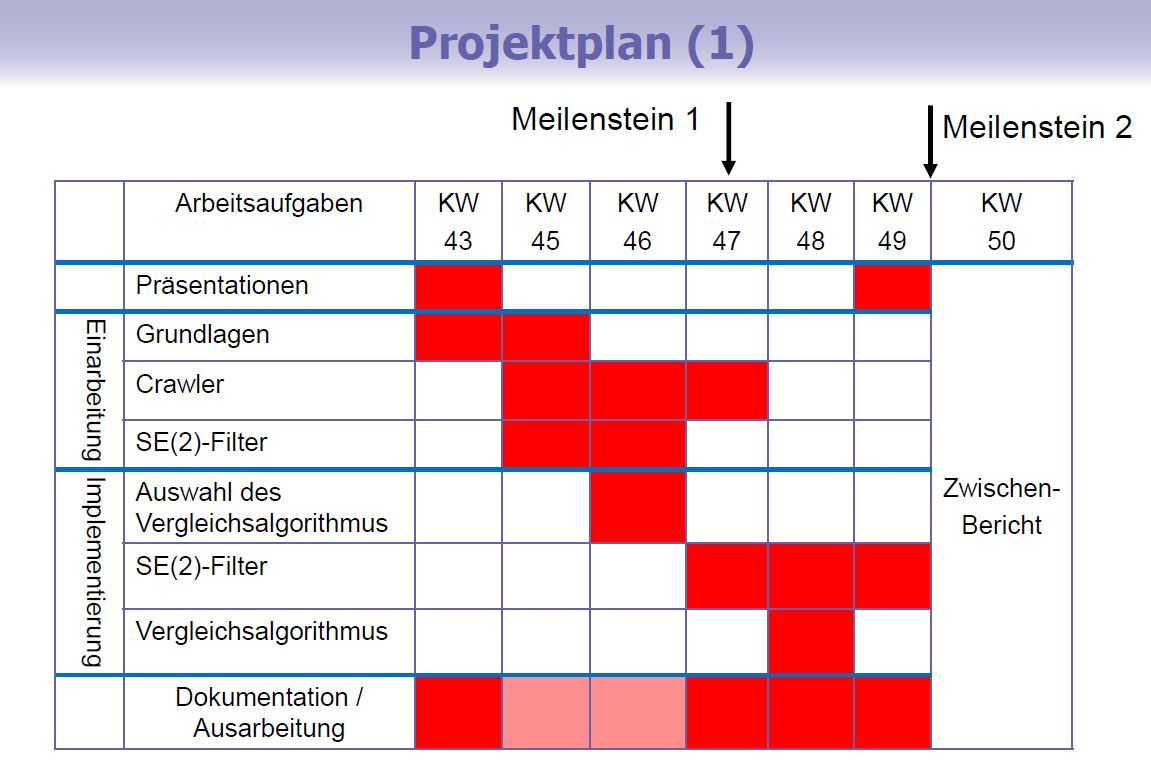
\includegraphics[width=0.9\linewidth]{Images/tu1}
	\caption{Zeitplaung 2017}
	\label{fig:tu}
\end{figure}

\begin{figure}[H]
	\centering
	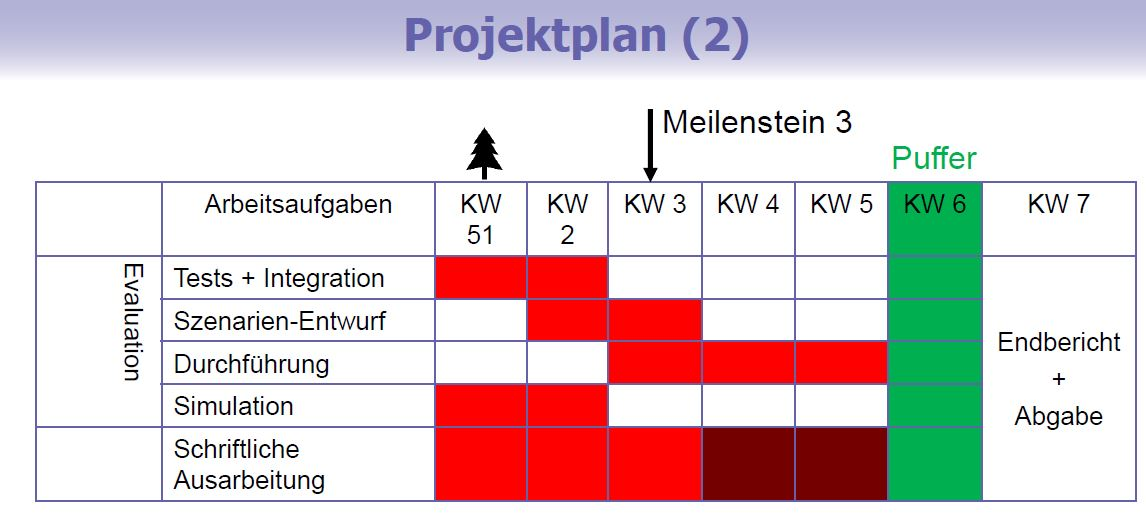
\includegraphics[width=0.9\linewidth]{Images/tu2}
	\caption{Zeitplannung 2018}
	\label{fig:tu2}
\end{figure}
\section{Schätztheorie}

\subsection{Bayes-Filterung}
Der allgemeinste Algorithmus zur Berechnung von Posterioren Wahrscheinlichkeiten, in unserem Projekt für die Position und Ausrichtung des Laufroboters, ist durch den Bayes-Filter gegeben.
 Dieser Algorithmus berechnet die Wahrscheinlichkeitsverteilung aus der Messung und Befehlen. Wir werden zuerst den grundlegenden Algorithmus mit den bisherigen Annahmen angeben. Eine Ablauf des Bayesfilterung-Algorithmus ist in der folgenden Abbildung dargestellt.

{\centering
 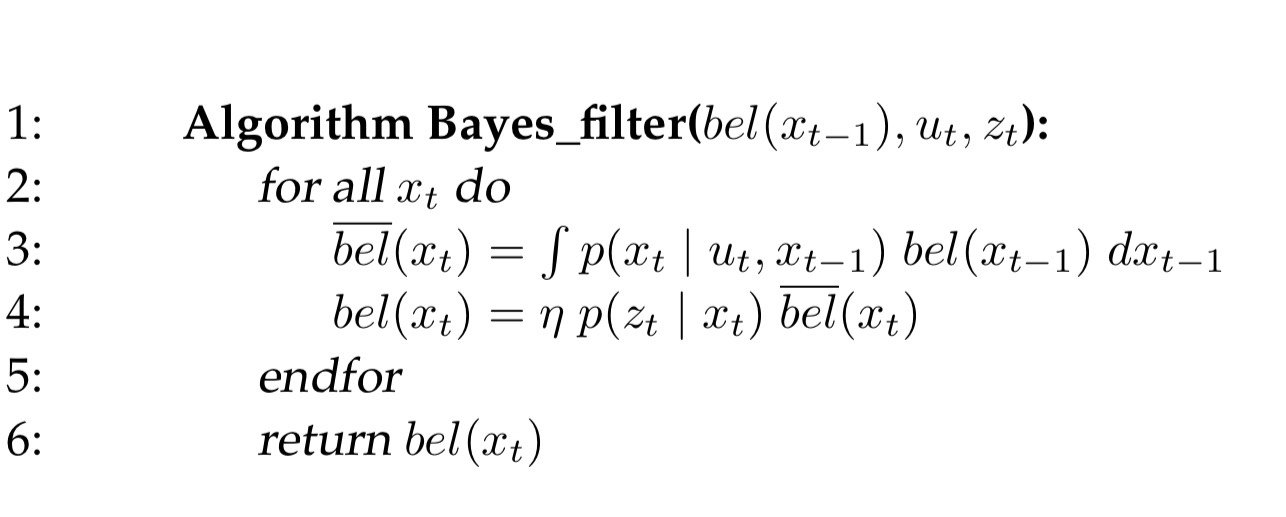
\includegraphics[width=12cm]{Images/image_6483441.jpg}}

Die gewünschte Ausgabe ist eine Schätzung des Zustands $bel(x_{t})$ zur Zeit $t$ (In unsere Projekt ist dies die Wahrscheinlichkeitsverteilung des aktuellen Zustands). Die Eingabe besteht aus der Schätzung des Vorgängerzustands $bel(x_{t-1})$, zusammen mit der letzten Befehl $u_{t}$ und der letzten Messung $z_{t}$. Die gesuchten Werte sind die Posterioren Wahrscheinlichkeiten $bel(x_{t})$ zum Zeitpunkt $t$. Dieser Updateschritt wird rekursiv angewendet. Erst wird das Schätzung $bel(x_{t})$ aus der Schätzung $bel(x_{t-1})$ zuvor berechnet. Deshalb besitzt die Bayes-Filter-Algorithmus aus zwei wesentlichen Schritten: Prediction und Update. Veranschaulicht in folgendem Diagramm.

{\centering
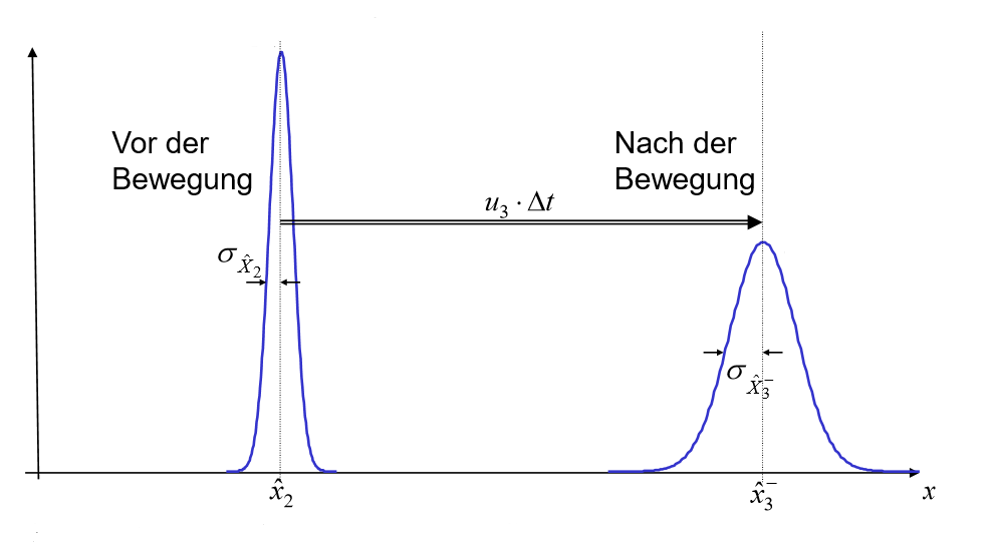
\includegraphics[width=8.2cm]{Images/prediction.png}}
{\centering
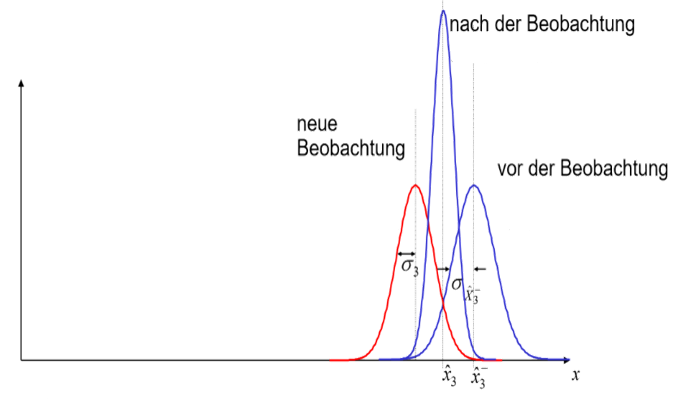
\includegraphics[width=8.2cm]{Images/update.png}}


\clearpage
\subsection{Kalman-filter}

Der Kalman-Filter dient dazu, Fehler in realen Messwerten zu reduzieren und Schätzungen für nicht messbare Systemgrößen zu liefern. Voraussetzung dabei ist, dass die interessierenden Werte durch ein mathematisches Modell beispielsweise in Form von Bewegungsgleichungen beschrieben werden können. Der Filter ermöglicht den Einsatz in Echtzeitsystemen verschiedener technischer Bereiche. Dazu zählen u.a. die Auswertung von Radarsignalen oder GPS-Daten zur Positionsbestimmung sich bewegender Objekte (Tracking). Deshalb ist er für unsere Projekt zur Positionschätzung geeignet. 
 
Das Kalman-Filter bestimmt wie das Bayes Filter seine Schätzungen rekursiv. Während das Bayes-Filter jedoch mit der Schätzfunktion jeweils die exakte Verteilung des aktuellen Zustands bestimmt, werden beim Kalman-Filter in jedem Schritt nur der Erwartungswert des Zustands und die Kovarianz dieser Schätzung bestimmt. Zur Initialisierung der Rekursion wird für $k = 0$ die Anfangsschätzung $\widehat{X}_{0}=X_0 $ mit der Kovarianz $P_{0}$ gewählt.Da der Kalman-Filter den Zustand eines Systems aus dem Eingangs- und Ausgangssignal schätzt, wird es als Zustandsschätzer bezeichnet. Das Kalman-Filter bestimmt zu jedem Zeitpunkt den Erwartungswert und die Kovarianz der zu schätzenden Größe. Die Berechnungsvorschrift wird nachfolgend hergeleitet.

\subsubsection{Prädiktionsschritt }
Im Prädiktionsschritt soll die beste Schätzung von $X_{k}$ und die zugehörigen Kovarianz aus der Befehlsfolge mit den zugehörigen Messungen $u_{1},...,u_{k},y_{1},...,y_{k-1} $ und $X_{0},P_{0}$ bestimmt werden. Außerdem ist die Schätzung des vorherigen Zeitschritts $\widehat{x}_{k-1}$ und deren Kovarianz $P_{k-1}$ verfügbar, welche die beste erwartungstreue Schätzung von $X_{k-1}$ unter Nutzung aller oben genannter Information außer $u_{k}$ darstellt.

Der Erwartungswert des Systemzustands wird mit Hilfe der Systemgleichung bestimmt wobei der unbekannte Zustand $X_{k-1}$ durch die aktuelle Schätzung $\widehat{x}_{k-1}$ ersetzt werden kann.

\begin{equation}
\tag{3.1}
\widehat{x}_{k}^{-}=E{X_{k}}=E{AX_{k-1}+Bu_{k}+R_{k}}
\end{equation}

Die Kovarianz der Prädiktion lautet damit
\begin{equation}
\tag{3.2}
{P}_{k}^{-}=Cov({X}_{k}^{-})=AP_{k-1}A^{T}+\Sigma_{R}
\end{equation}

In der Umformung wurde genutzt, dass das Systemrauschen zum Zeitpunkt $k$ unkorreliert mit
Größen vorheriger Zeitpunkte ist. Der erste Summand der Kovarianz gibt die in Schritt $k-1$ bestehende
Unsicherheit gewichtet mit der Systemdynamik A wieder. Durch den zweiten Summanden
kommt noch das neue Systemrauschen $R_{k}$ hinzu. Gleichungen $(3.1)$ und $(3.2)$ bestimmen somit, wie aus der Schätzung des Systemzustands und deren Kovarianz zum vorherigen Zeitpunkt$ k-1$ eine Prädiktion derselben Größen für den Zeitpunkt k.

\subsubsection{Innovationsschritt}
Im Innovationsschritt soll zusätzlich die aktuelle Beobachtung $y_{k}$ berücksichtigt werden. In dieser Schritt wird erst die Verstärkungsmatrix (Kalman Gain) berechnet:

\begin{equation}
\tag{3.3}
K=\widehat{P}_{k}^{-}C^{T}(CP_{k}^{-}C^{T}+\Sigma_{S})^{-1}
\end{equation}
Entsprechend erfolgt die Innovation linear, als gewichtete
Summe der aktuellen Schätzung und einer Innovation, die proportional zum aktuellen Beobachtungsresiduum ist
\begin{equation}
\tag{3.4}
\widehat{x}_{k}=\widehat{x}_{k}^{-}+K(y_{k}-C\widehat{x}_{k}^{-})
\end{equation}
Unter Nutzung der Voraussetzung, dass das Beobachtungsrauschen $S_{k}$ unkorreliert ist mit der Prädiktion, lässt sich die Kovarianz der Innovation berechnen gemäß

\begin{equation}
\tag{3.5}
P_{k}=(I-KC)P_{k}^{-}(I-KC)^{T}+K\Sigma_{S}K^{T}
\end{equation}
Wie noch gezeigt wird, lässt sich dieser Ausdruck für die optimale Verstärkungsmatrix des KalmanFilters K weiter vereinfachen zu

\begin{equation}
\tag{3.6}
P_{k}=(I-KC)P^{-}_{k}
\end{equation}


\subsection{Partikel-Filter}
Als Vergleichsverfahren für den SE(2)-Filter wird der Partikel-Filter verwendet. Partikel-Filter ist auch als SMC-Methode bekannt. Die Funktionsweise der Filterung ebenfalls auf der Bayes-Filterung. Der Partikelfilter ist eine alternative nichtparametrische Implementierung des Bayes-Filter. Partikelfilter nähern sich der posterioren Wahrscheinlichkeit an. 
Es wird eine große Anzahl an Partikeln mit verschiedenen Parametern zu generiert und in dem den Zustandsraum zu füllen ist die Schlüsselidee.
Die Posteriori Schätzung $bel(x_{t})$ soll durch eine Zufallsmenge dargestellt werden. Von dieser posterioren Verteilung werden Zustandsproben gezogen. Anstatt die Verteilung durch eine parametrische Form darzustellen, stellt der Partikelfilter die Verteilung durch eine Menge von Stichproben aus der aktuelle Verteilung dar. Die ganze Prozess kann durch folgendes Diagramm veranschaulicht werden.

    {\centering
    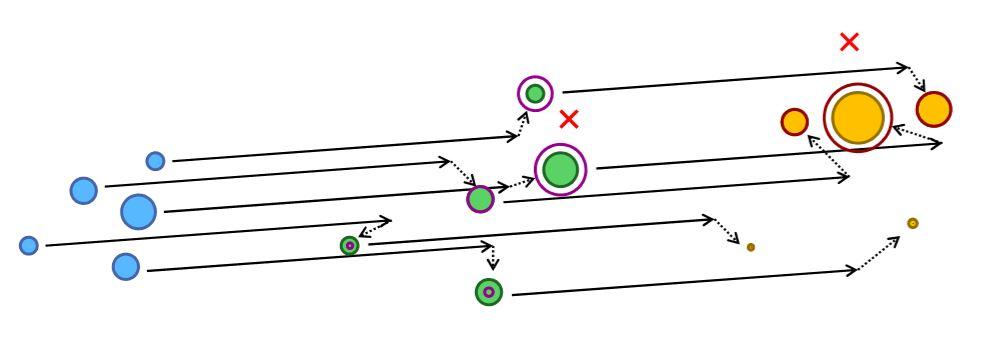
\includegraphics[width=15cm]{Images/pf.jpg}}
    
Das oben gezeigtem Bild beschreibt den Prediction- und Update-Schritt des Partikelfilters. Die blauen Partikel ist die Stichproben des aktuellem Zustands, durch die Zustandsüberführung werden die Partikel für den nächsten Schritt erzeugt (in Bild sind dies die grünen Partikel), im nächsten Schritt werden die Partikel durch die aktuelle Messungen korrigiert. Daraus bekommen wir posteriore Stichproben.
In unsere Projekt wird die Partikel-Filter durch die PF-Klasse von robotics system toolbox eingesetzt. Damit können wir direkt das Systemmodell für die Zustandüberführung und das Messmodell des Partikel-Filter anpassen.
\section{SE(2) Filter}

\subsection{Lie Gruppe}
 Eine Lie-Gruppe G ist eine Mannigfaltigkeit G, welche zusammen mit einer glatten Operation 
 
 \begin{equation*}
  G\times G\ni (g_{1},g_{2})\to g_{1}\cdot g_{2}\in G
 \end{equation*}
eine Gruppe ist.


Ein Vorteil der abstrakten Definition von Lie-Gruppe besteht darin, dass sie wesentlich flexibler ist. Zum Beispiel gilt folgendes: Ist G eine Lie-Gruppe und N ein abgeschlossener Normalteiler, dann ist G/N wieder eine Lie-Gruppe.


\subsection{SE(2)-Bingham-Verteilung}
In diesem Projekt verwenden wir einen Filter, der auf der SE(2)-Bingham-Verteilung für zweidimensionale Translationensvektoren und einem Skalar für die Rotation basiert. Die SE(2)-Bingham-Verteilung kann zur Darstellung der Orientierungen auf der Ebene verwendet werden. [5]
Anstatt sich auf die auf Gauß'sche-Verteilung basierende Annäherungen zu verlassen, haben wir uns entschieden, alle auftretenden Wahrscheinlichkeiten durch SE(2)-Bingham-Verteilung darzustellen. Diese verwendet für die Translation weiterhin eine zweidimensionale Normalverteilung, kombiniert mit einer Bingham-Verteilung, die auf der Hypersphere der Rotationen definiert wird. Die  antipodisch Symmetrie ist in Abbildung \ref{fig:bingham} gezeigt.

\begin{figure}
	\centering
	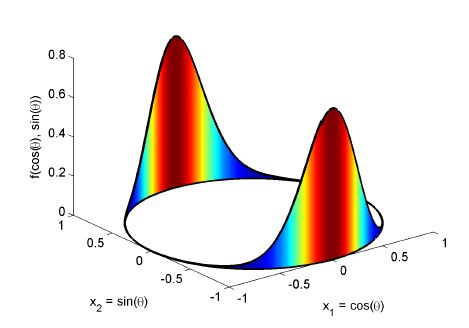
\includegraphics[width=0.7\linewidth]{Images/bingham}
	\caption{Darstellung von hypersphärischen Zufallsvektoren [2] }
	\label{fig:bingham}
\end{figure}

In unsere Fall ist die Bingham-Verteilung einfacher für die Darstellung der Orientierung des Laufroboters. Als eine Folge der obigen Motivation kann man sehen, dass die Bingham- Wahrscheinlichkeits- dichtefunktion (pdf) zwei symmetrische Moden aufweist. Die Parametermatrix der Bingham-Verteilung aus der Exponentialfunktion  (welche die inverse  Kovarianzmatrix im Gauß'schen Fall ist) wird üblicherweise zerlegt in eine orthogonale und eine diagonale Matrix. Dies führt zu der folgenden Definition:
\begin{equation}
	f\left(\vec{x}\right)=\frac{1}{F}\cdot exp\left(\vec{x}^{T}MZM^{T}\vec{x}\right)
\end{equation}




\subsection{Duale Quaternionen}
In unsere Projekt werden duale Quaternionen zur Darstellung der Starrkörperbewegung verwendet. Die dualen Quaternionen werden durch folgende Formel darstellt [1]

\begin{equation}
\sigma=p+\epsilon q
\end{equation}
Unter Ihnen die p steht für jeweilige Quaternionen
\begin{equation}
	p=p_{0}+\vec{p}=p_{0}+p_{1}\vec{i}+p_{2}\vec{j}+p_{3}\vec{k}
\end{equation}
\begin{equation}
	q=q_{0}+\vec{q}=q_{0}+q_{1}\vec{i}+q_{2}\vec{j}+q_{3}\vec{k}
\end{equation}
Für die duale Einheit $\epsilon$ gitl $\epsilon^2 = 0$.

Die Rotationsmatrix R, Translationsvektor t kann kompakt durch eine duales Quaternion dargestellt werden. Der Translationsvektor t ist ein reines Quaternion. Wir kombinieren es mit dem Rotationsquaternion $r =\cos\frac{\theta}{2}+ \vec{\widehat{u}}sin\frac{\theta}{2}$, das die Rotation um den Vektor $\widehat{u}$ beschreibt, zu dem folgendem dualem Quaternion:

\begin{equation}
	\sigma = r + \frac{\epsilon}{2}\vec{t}r\\
	=cos\frac{\theta}{2}+ \vec{\widehat{u}}sin\frac{\theta}{2} + \frac{\epsilon}{2}\left( -sin\frac{\theta}{2}\left(\vec{t}\cdot\widehat{u} \right)+ cos\frac{\theta}{2} \vec{t}+sin\frac{\theta}{2} \vec{t} \times \widehat{u} \right) 
\end{equation}

In unseren Fall wird die Bewegung der Roboter hauptsächlich auf eine Eben durchgeführt werden. Deshalb stehen $\vec{t}_{x}$ und $\vec{t}_{y}$ für die Translation des Roboters und $\theta$ für die Rotation. Um Rotationen und Translationen in 2D zu kombinieren, wird hier
duale Quaternion-Multiplikation verwendet. Eine Rotation mit anschliesender Translation wird durch die Multiplikation beschrieben.
\begin{equation}
	\left[1+\epsilon\frac{1}{2}\left(t_{x}\vec{i}+t_{y}\vec{j}\right) \right] \cdot\left[cos\left( \frac{\alpha}{2}\right)+sin\left(\frac{\alpha}{2}\right)\vec{k}\right]
\end{equation}

\section{Crawler}
In unsere Projekt wird ein Laufroboter verwendetder vom Labor für Intelligente Sensor-Aktuator-Systeme (ISAS) selbst aufgebaut wurde. Es bestehen viele verschiedene Versionen des Crawlers. Diese Roboter werden für mehrere Zwecke verwendet. Darüber hinaus ist das Chassis von diesen
Roboter komplett in 3D gedruckt. Daher können diese sehr schnell gebaut werden.


\begin{figure}[b!]
	\centering
	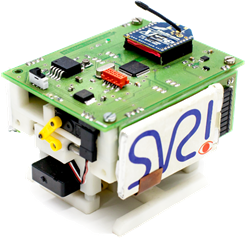
\includegraphics[width=0.5\linewidth]{Images/crawler}
	\caption{Der Crawler}
	\label{fig:crawler}
\end{figure}

\subsection{Aufbau}
Der Crawler, der im Projekt benutzt wird, ist die neueste Version. Die Hauptkomponente der Version ist ein Arduino Yun.
\\Der Arduino Yun verfügt über ein WLAN-Modul, mit dem ein WLAN generiert Oder in ein bestehendes WLAN eingefügt wird. Der Craeler verfügt es über drei verschiedene Beine, wobei jedes einzeln mittels Servomotor gesteuert werden kann. Dies ermöglicht dem Roboter, sich gerade, seitlich und omnidirektional zu bewegen.
\\Der Crawler enthält vier Ultraschallsensoren und eine IMU. Es sind insgesamt vier Ultraschallsensoren installiert, die jeweils aus einem bestehen Empfänger und ein Sender existieren.  Die Sensoren sind in 90-Winkeln zueinander angeordnet
\\Zusätzlich befinden sich oben zwei LEDs (gelb und rot), mit denen der
Roboter einfacher, zum Beispiel von einer Deckenkamera, verfolgt werden kann.
Das Design der Roboter ermöglicht eine Vielzahl unterschiedlicher Grundfunktionen Bewegungsmuster.










\subsection{Position- und Rotationschätzung mittels Kameratracking}
Zur bessere Simulation und Evaluierung muss die genau Position und Rotation ermittelt werden. Dazu wird ein Deckenkamerasystem verwendet. Zur Ermittelung der Position unseres Laufroboters wird ein rote LED auf dem Crawler aktiviert, die durch das an der Decke befestigte Kamerasystem aufgenommen wird. Durch eine Farberaum-Umwandlung kann die rote Markierung im Bild zuverlässig gefunden werden. Mittles anschließender  Koordinatentransform, die und Gleichung \ref{fig:coordinates} gezeigt ist,  wird die Position des echten Crawlers ermittelt und umgewandelt.
Für die Rotation wird entsprechend eine zweite gelbe LED in Crawler eingesetzt, durch den bekannten Aufbau kann die Bewegungsrichtung durch das Kamerasystem erkannt werden. Die gesammelten Bewegungsdaten können zusammen mit den Messdaten des Crawlers als Ground Truth exportiert werden. Das ganze Prozess wird durch unten stehend Bild dargestellt.

\begin{figure}
    \centering
    \left[ \begin{array}{c}
    x_{k+1} \\ 
    y_{k+1} \\ 
    \Phi_{k+1}
    \end{array} \right] =\left[ \begin{array}{c}
    x_{k} \\ 
    y_{k} \\ 
    \Phi_{k}
    \end{array} \right]+\left[ \begin{array}{ccc}
    cos(\Phi_{k}) & -sin(\Phi_{k}) & 0 \\ 
    sin(\Phi_{k}) & cos(\phi_{k}) & 0 \\ 
    0 & 0 & \Phi_{k}
    \end{array} \right] \left[ \begin{array}{c}
    \widehat{s}_{k}^{F} \\ 
    \widehat{s}_{k}^{S} \\ 
    \widehat{\omega}_{k}
    \end{array} \right] +\left[ \begin{array}{c}
    \omega_{k}^{x} \\ 
    \omega_{k}^{y} \\ 
    \omega_{k}^{\Phi} \\
    \end{array} \right] \\
    \caption{Umwandlung in Crawlerkoordinaten}
	\label{fig:coordinates}
\end{figure}


\begin{figure}
	\centering
	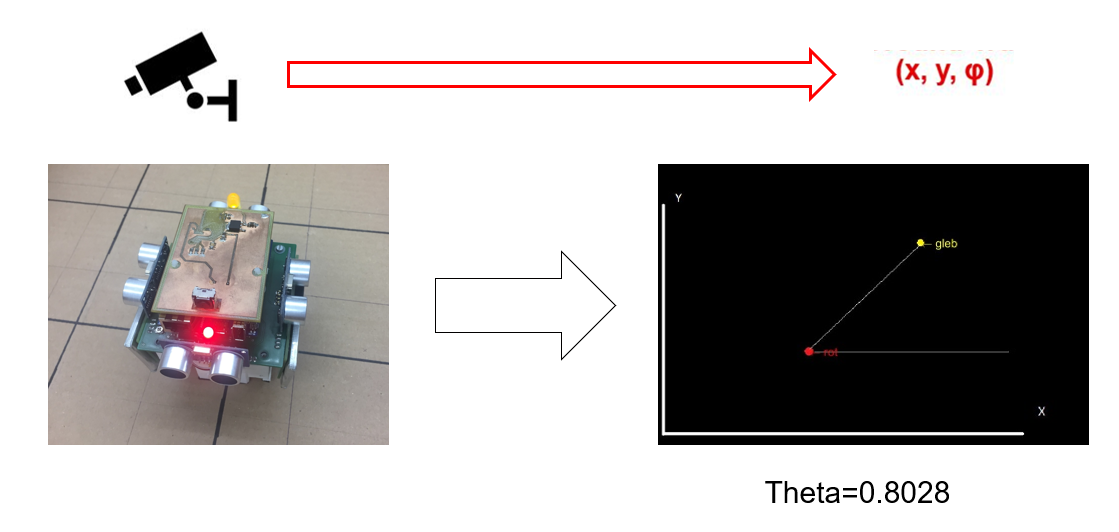
\includegraphics[width=0.9\linewidth]{Images/camera.png}
	\caption{Erkennung der LEDs aus dem Kamerabild, zum Tracking des Laufroboters.}
	\label{fig:crawler}
\end{figure}

\begin{figure}
	\centering
	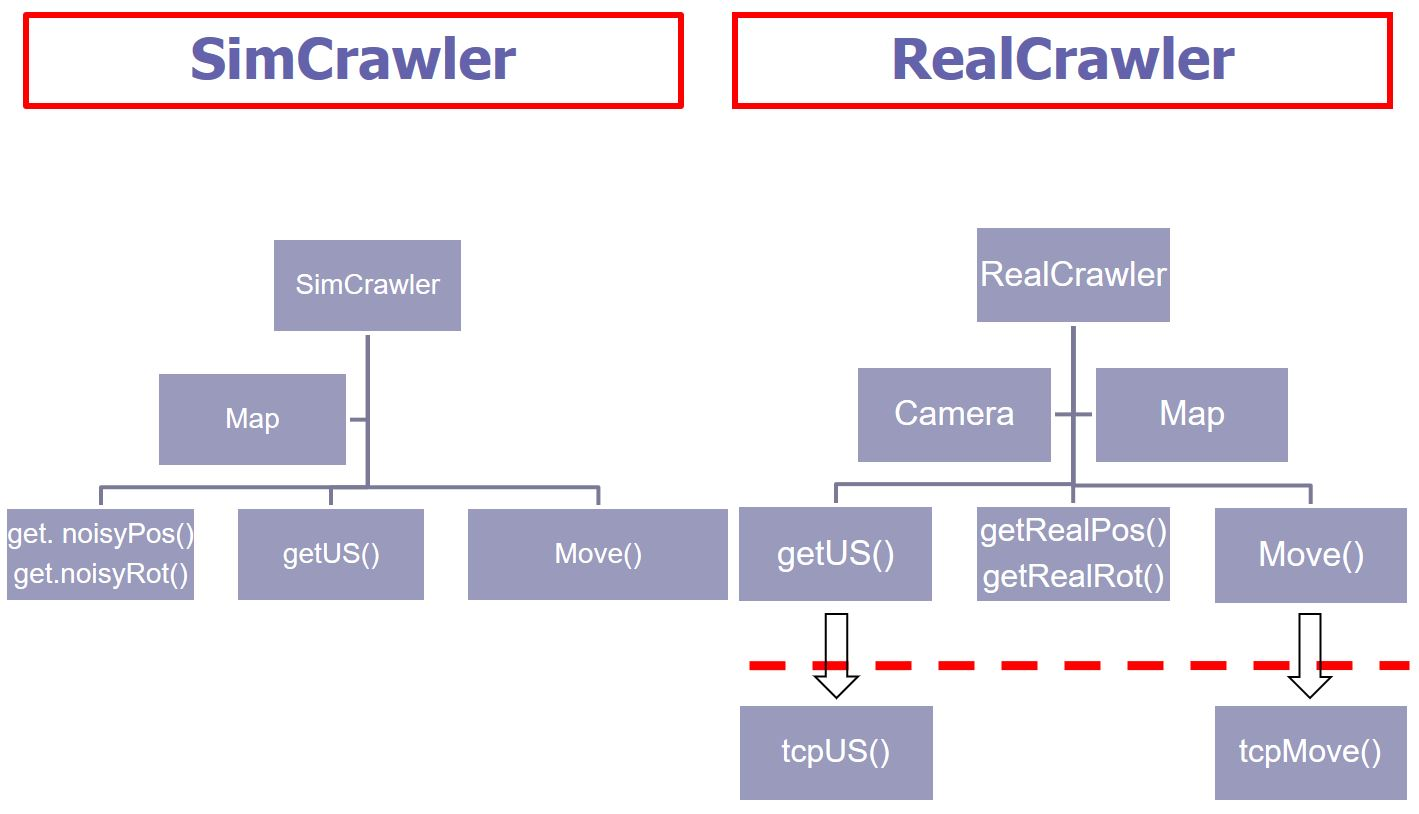
\includegraphics[width=0.9\linewidth]{Images/crawlerklass.jpg}
	\caption{Gemeinsam genutzte Schnittstelle der Crawler-Klassen}
	\label{fig:crawler}
\end{figure}
\clearpage

\section{Simulation}
Zur Überprüfung der Implementierung wurde die Bewegung des Crawlers zunächst simuliert. Die Simulation bietet ein Ground Truth ohne aufwändiges Kameratracking vorteilhaft, sowie verschiedene Karten. Diese können als beliebige konvexe Polygone definiert werden, in denen sich der Crawler frei bewegen kann.
Um Komponenten der Simulation zur Auswertung des Experiments wiederverwenden zu können, wurde auf einen modularen Aufbau geachtet. Die grobe Struktur des Frameworks wird in \ref{fig:class} verdeutlicht. Es gibt eine einheitliche Schnittstelle, die zur Kommunikation mit der realen Crawler-Hardware, sowie dem simuliertem Crawler genutzt wird. Die Steuerung ist über drei verschiedene Modi möglich:
\begin{itemize}
	\item Auswahl der Bewegungsanweisungen durch den Benutzer
	\item Zufällige Bewegungsanweisungen
	\item Wiedergabe eines aufgezeichneten Bewegungspfads des echten Crawlers
\end{itemize}

\begin{figure}
	\centering
	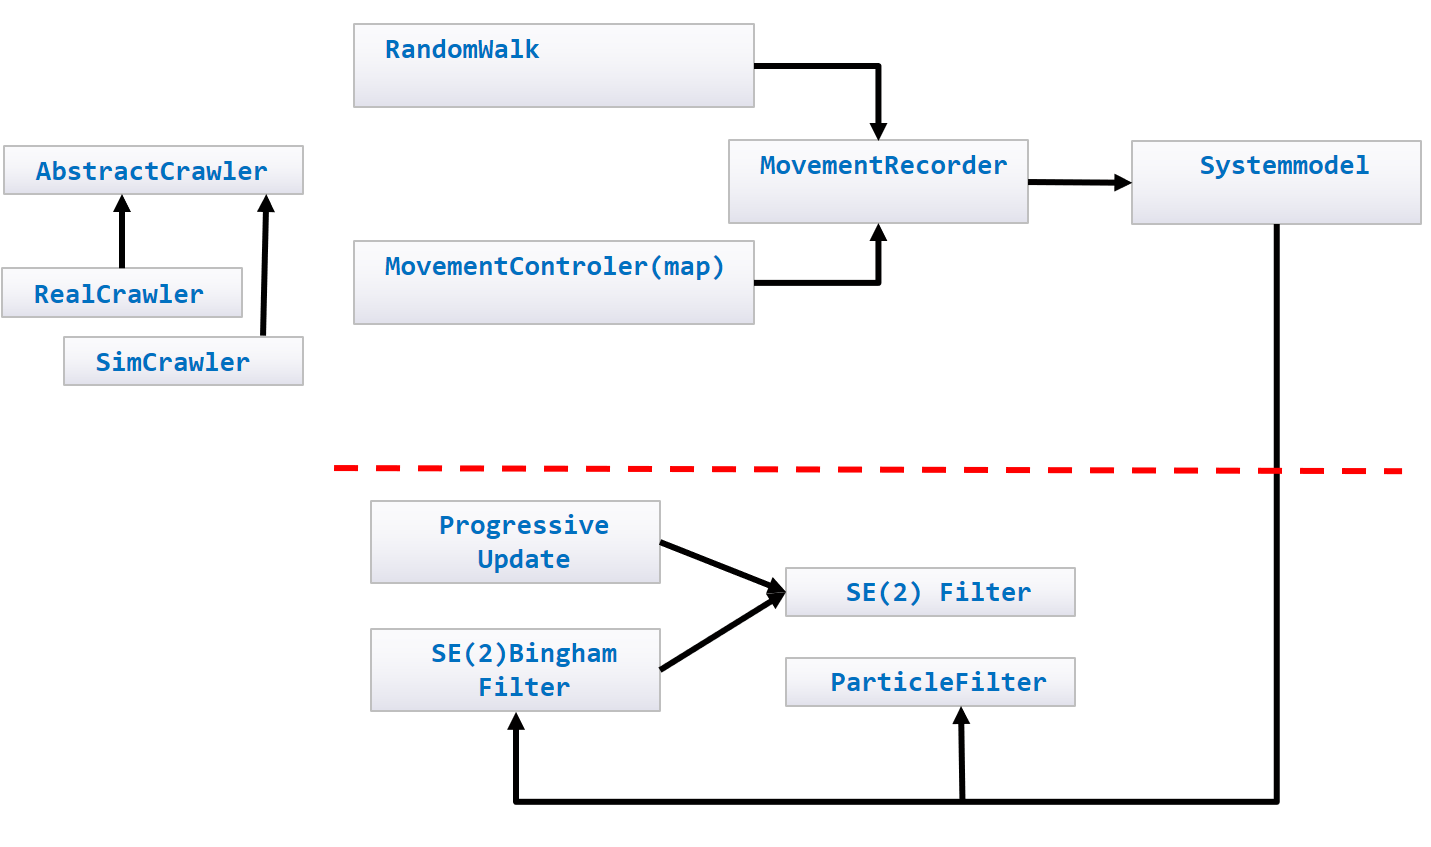
\includegraphics[width=0.9\linewidth]{Images/class.png}  
	\caption{Aufbau des Simulationsframeworks}
	\label{fig:class}
\end{figure}

Crawler Modell
Das vereinfachte Modell des Crawlers, das zur Simulation verwendet wurde ist in \ref{fig:ModelCrawler} zu sehen. Der Ursprung des Koordinatensystems liegt auf der vorderen roten LED, die zum Tracking der Position verwendet wurde. Der eigentlich kegelförmige Messbereich der vier Ultraschallsensoren wurde als Halbgerade modelliert.

\begin{figure}[ht]
	\centering
	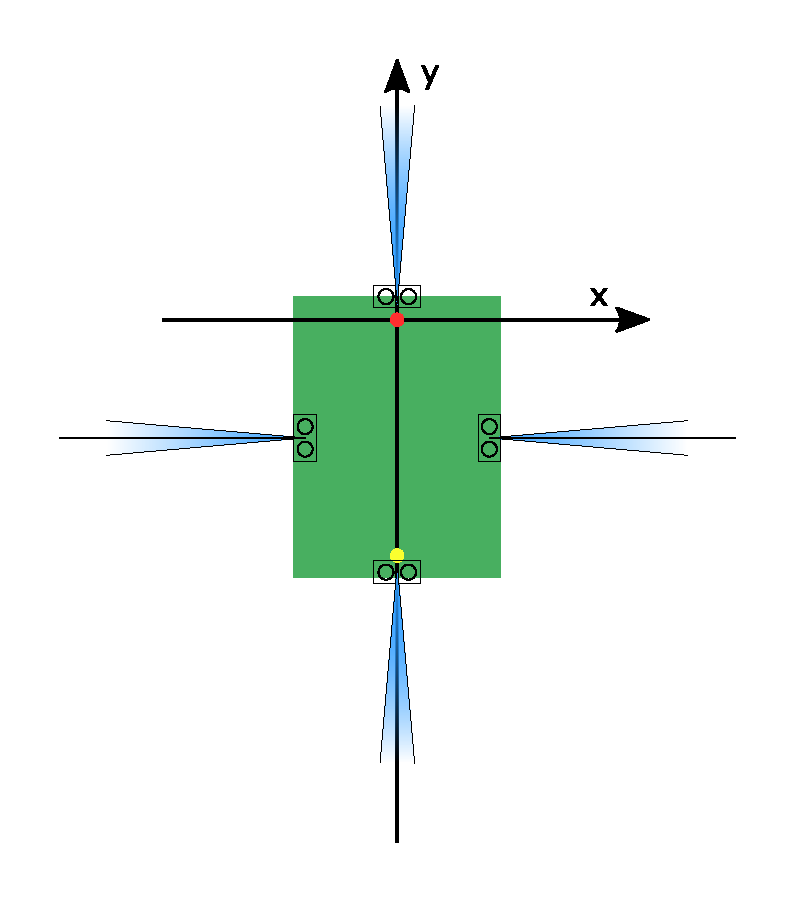
\includegraphics[]{Images/ModelCrawler}  
	\caption{In der Simulation verwendetes Schema des Crawlers mit lokalem Koordinatensystem. Markeirt sind die vier Ultraschallsensoren mit Messbereich, sowie die zwei verschiedenfarbenen LEDs.}
	\label{fig:ModelCrawler}
\end{figure}

\subsection{Systemmodell}
Vorwissen über das System findet im Systemmodell Anwendung. Mit der Überführungsfunktion $a$ wird der Folgezustand $\vec{x}_{t+1}$ aus dem aktuellem Zustand $\vec{x}_t$ abgeleitet. Der verwendete Zustandsraum $\mathbb{S} \times \IR^2$ beschreibt die position und Orientierung des Crawlers.


\begin{align*}
\vec{x}_{t+1} = a(\vec{x}_t) \oplus w_t
\end{align*}

Die Folge von Bewegungsbefehlen an den Crawler ist bekannt. Je nach Bewegungsbefehl ist die entsprechende Überführungsfunktion zu wählen:

\begin{equation}
    a(\vec{x}_t, command) = 
        \begin{cases}
            a_{fwd} \oplus w_{fwd},& \text{falls } command= fwd \\
            a_{left} \oplus w_{left},& \text{falls } command= left\\
            a_{right} \oplus w_{right},& \text{falls } comman= right
        \end{cases}
\end{equation}

Die tatsächliche ausgeführten Schritte variieren jedoch, auch für gleichbleibende Bewegungsrichtungen. Dies wir in Abbildung \ref{fig:moves} deutlich. Deswegen wird bei jedem Schritt zusätzlich ein Rauschterm $w_t$ addiert. Dies lässt sich in SE(2) durch die Multiplikation der dualen Quaternionen darstellen, was durch den $\oplus$-Operator ausgedrückt wird.
Die Schrittlängen und Drehungen wurden in einem Vorexperiment durch Tracking der LEDs mit der Deckenkamera aufgenommen. Es wurden drei SE(2)-Bingham-Verteilungen auf die gewonnen Daten angepasst, aus denen die jeweiligen $w_t$ zufällig gezogen werden.





\begin{figure}[ht]
	\centering
    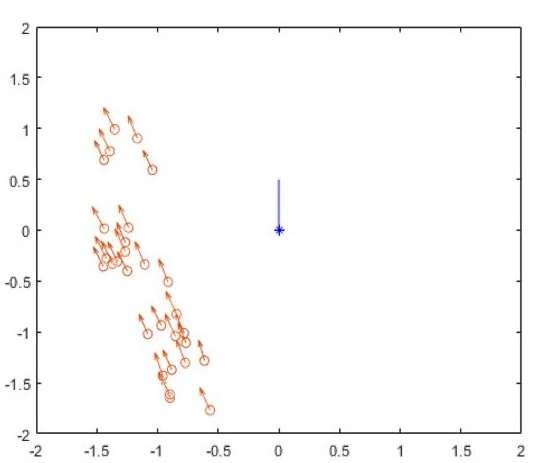
\includegraphics[width=.32\textwidth]{Images/links.jpg}
    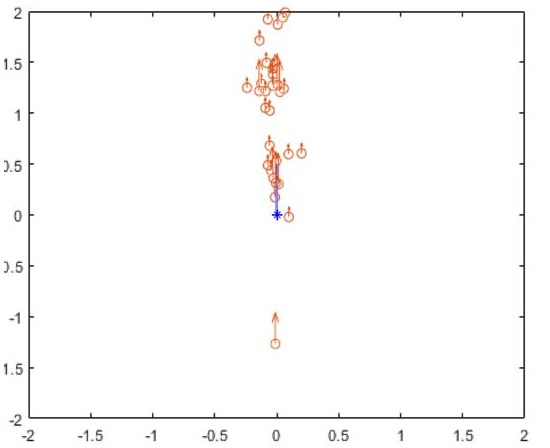
\includegraphics[width=.32\textwidth]{Images/vorne.jpg}
    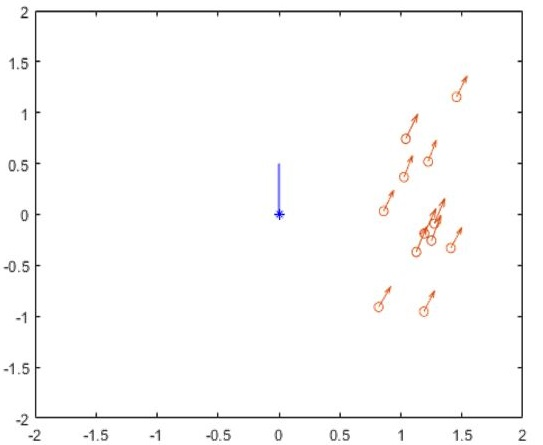
\includegraphics[width=.32\textwidth]{Images/rechts.jpg}
	\caption{Gemessene Verteilungen der Position und Rotation des Laufrobotters nach der Ausführung einer Bewegung. Blau ist der Ausgangszustand dargestellt. Die Zustände nach je einem Schritt in rot. Jede Verteilung wurde für einen der drei Bewegungsbefehle 'links', 'vorwärts' und 'rechts' mit einer Deckenkamera gemessen.}
	\label{fig:moves}
\end{figure}

Daraus werden die Erwartungswert und Varianz berechnet,und wir bezeichnen diese Datensätze als die echte Systemrauschen von Roboter.

\subsection{Messmodell}

Der Crawler kann seine momentane Position und Ausrichtung nicht direkt messen. Es stehen jediglich vier nach vorne, hinten, links und rechts gerichtet Ultraschallsensoren zur Verfügung, die Abstandsmessungen zu den nächstliegenden Wänden vornehmen könne. Die Messwerte hängen bei einer festen Karte von der Position und Ausrichtung des Crawlers ab. 
Mit dem Messmodel wird beschrieben, welche Messergebnisse bei einem Systemzustand zu erwarten sind. Eine Messung ist Abbildung vom dreidimensionalen Zustandsraum des Laufroboters $\mathbb{S} \times \IR^2$ in einen vierdimensionalen Messraum ${\IR^+}^4$.

Da die Ultraschallsensoren des Crawler nur grobe Abstandsmessungen ermöglichen, wird ein normalverteiltes mittelwertfreies Rauschen $w_t \sim \mathcal{N}(0,\sigma)$ addiert:

\begin{align*}
\vec{z}_{t} = h(\vec{x}_t) \oplus w_t
\end{align*}

$h(x_t)$ für einen Zustand $x_t$ zu berechnen ist leicht. Es muss lediglich eine Messung auf einer virtuellen Karte an der von $x_t$ beschriebenen Position durchgeführt werden. In unserem Fall lässt sich $h$ jedoch nicht einfach invertieren. $h^{-1}$ muss nicht eindeutig sein. Die selbe Messung könnte kann in mehreren verschiedenen Zuständen beobachtet werden.
Aus $h$ lässt sich ohne weiteres die eine Likelihood $f(z_t | x_t)$ ableiten [3]. Diese beschreibt die Plausibilität einer Messung für einen gegebenen Zustand. Die Likelihood kann folgendermaßen berechnet werden $f(z_t | x_t) = f_{\mathcal{N}}(h(x_t)  - z_t)$, wobei  $f_{\mathcal{N}}$ komponentenweise in eine Normalverteilung $\mathcal{N}$ einsetzt und die resultierenden Wahrscheinlichkeiten multipliziert. Die Abbildung \ref{fig:likelihood} zeigt den Crawler in der Position im linken Bild, mit der Likelihood-Funktion für den gezeigten Zustand rechts. Der hell gelbe Punkt rechts, mit der größten Wahrscheinlichkeit befindet sich an der Stelle des Crawlers, von dem die Messung $z_t$ stammt.

\begin{figure}[ht]
	\centering
	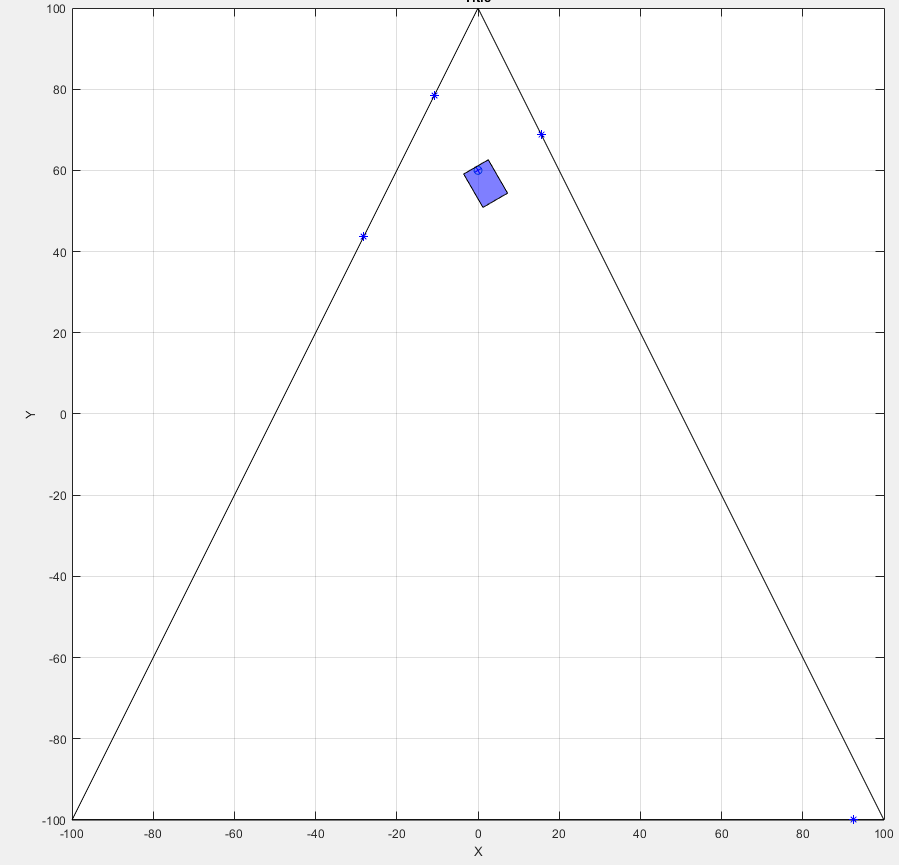
\includegraphics[width=8cm]{Images/likelihoodPosition.png}
    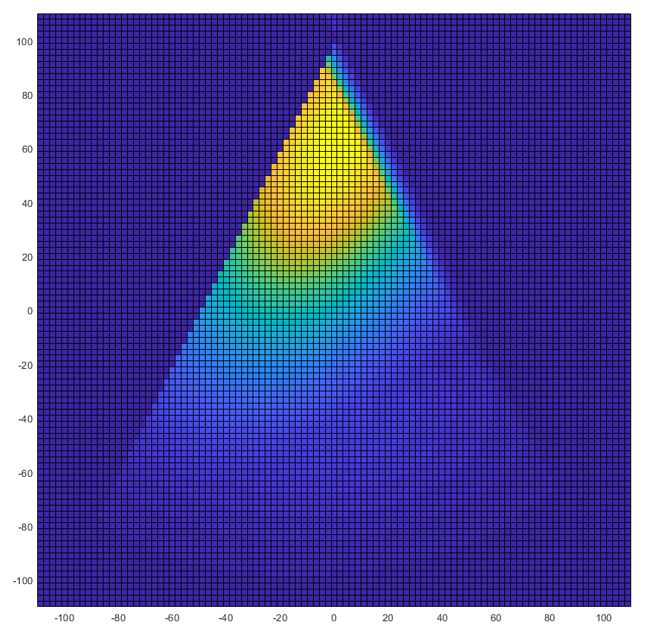
\includegraphics[width=8cm]{Images/likelihood.jpg}  
	\caption{Linkes Bild: In blau ist der Crawler auf der dreieckigen Karte eingetragen. Rechts die Likelihood-Funktion $f(z_t | x_t)$, für die Messung, die der Crawler im linken Bild aufnimmt.}
	\label{fig:likelihood}
\end{figure}

\subsection{Progressive Updates}

Nach Anwendung des Systemmodells im Prediction-Schritts folgt  der Aktualisierungsschritt, der den geschätzten Zustand $x_{t}^{e}$ durch Einbeziehung der Messung $z_{t}$ korrigiert
Beim Progressiven Update werden vom aktuell geschätze Systemzustand $x_{t}^{e}$ dazu zunächst deterministisch Proben gezogen. Anstatt diese in einem Schritt mit den Werten der Likelihood-Funktion neu zu gewichten, wird iterativ vorgegangen [4]. Dies ist nach der Regel von Bayes möglich, wenn die $\lambda_1 + \lambda_s$ eine Zerlegung der $1$ bilden. Dadurch kann eine Degenerierung der Proben mit Likelihoodwerten nahe null vermieden werden. Degenerierte Proben verringern die Genauigkeit des Filters. Außerdem ermöglicht das Progressive Update die Korrektur des geschätzten Orts ohne die Messfunktion $h$ invertieren zu müssen. Gemessene Werte können direkt in die Likelihood eingesetzt werden.

\begin{align*}
	f(\vec{x} | \vec{z}) \propto f(\vec{z} | \vec{x}) * f(\vec{x})\\
	= (f(\vec{z} | \vec{x})^{\lambda_1} * ... * f(\vec{z} | \vec{x})^{\lambda_s}) * f(\vec{x})
\end{align*}


 Durch den folgenden Ablauf wird garantiert, dass der Quotient zwischen dem kleinsten neuen Gewicht
$l_{min}$ und das größte neue Gewicht $l_{max}$ nicht über einen vorbestimmten Schwellwert steigt. Dieser Schwellwert wird mit $\tau$ bezeichnet.
\\

\begin{alogrithm}
	\caption{Ablauf des Progressiven Updates}\label{update}
	\begin{algorithmic}[1]
		\Procedure{Update}{measurement $z_t$, likelihood $f(z_t | x_t)$, predicted density $x_{t}^{e}$}
	  \State $\Lambda\leftarrow 1$
	  \State $x_{t} \leftarrow x_{t}^{e}$
	  \While{ $\Lambda>0$ }
	  \State $(s_{1},...,s_{L},\omega_{1},...,\omega_{L})\leftarrow \text{sampleDeterministicly}(x_t)$
	  \State $\omega_{min}\leftarrow min(f(z_{k}|s_{k}))$
      \State $\omega_{max}\leftarrow max(f(z_{k}|s_{k}))$
	  \State $\lambda \leftarrow min(\Lambda, \frac{log(\tau)}{log(\omega_{min}/\omega_{max})})$
	  \For{$j \leftarrow 1 \textbf{to} L$}
		\State $\omega_{k} \leftarrow \omega_{k}\cdot f(z_{k}|x_{k})^{\lambda}$
      \EndFor
	  \State $x_t \leftarrow matchBingham(s_{1},...,s_{L},\omega_{1},...,\omega_{L})$
	  \State $\Lambda\leftarrow\Lambda-\lambda$
    \EndWhile
	\EndProcedure
  \end{algorithmic}

\end{alogrithm}



\clearpage
\section{Evaluation}

Zur Evaluierung wurde der Crawler auf einer einfachen rechteckigen Karte zufällig bewegt. Dabei wurde aus drei Bewegungsmöglichkeiten nach Tabelle \ref{tab:vars} probabilistisch eine ausgewählt, und ausgeführt, sofern dies ohne eine Kollision des Crawlers mit der Wand möglich ist. Die Position und Orientierung des Laufroboters werden parallel vom SE(2)-Filter und Partikelfilter geschätzt. Dann wird jeweils der Fehler zum Ground Truth berechnet. Für den Partikelfilter wurden 1000 eingesetzt, die Rotationskoordinate wurde in $mathtbb{S}$ berechnet.
In den Anfangsverteilungen wurden jeweils alle Koordinaten als stochastisch unabhängig voneinander angegeben.

\begin{table}[h!]
	\centering
	\caption{Mögliche Bewegungen}
	\label{tab:vars}
	\begin{tabular}{lll}
		\toprule
		Notation & Erklärung & Wahrscheinlichkeit\\
		\midrule
		$fwd$ 	& Schritt gerade nach vorne & 50\%\\
		$left$	& Drehung nach links		& 25\%\\
		$right$	& Drehung nach rechts		& 25\%\\

		\bottomrule
	\end{tabular}
\end{table}

Als Ground Truth wird der Crawler mit einer Deckenkamera getrackt. Über zwei verschiedenfarbige LEDs auf dem Crawler lässt sich dessen Position und Rotation bestimmen.

Aufgrund des hohen Zeitaufwands für das Aufnehmen von Bewegungspfaden des echten Crawlers, wurden zusätzlich in der Simulation erstellte zufällige Bewegungspfade als Ground Truth verwendet. Hierbei gibt es mehrere Möglichkeiten, welche Verteilung für das Rauschen im Systemmodell verwendet wird. Um den SE(2)-Filter nicht zu bevorteiligen, wenn im Systemmodell genau die Bingham-Verteilung des Filters verwendet wird, wurde eine weitere Testreihe mit Normalverteiltem Rauschen durchgeführt. Die hierfür benötigten Mittelwerte und Varianzen wurden für jeden der drei Freiheitsgrade $x,y,\theta$ unabhängig aus den Messdaten des Vorexperiments bestimmt.
Tabelle \ref{tab:testreihen} zeigt die insgesamt sechs Kombinationen aus den zwei Verfahren und drei Ground Truths. Für die Simulationen wurden die drei Karten aus Abbildung \ref{fig:map} mit jeweils 100 zufälligen Schritten betrachtet. Die Bewegungsbefehle waren für beide Verfahren pro Karte gemeinsam generiert. Für den realen Versuch wurde nur die quadratische Karte untersucht, mit zwei Bewegungsmustern von 60 und 40 zufälligen Schritten, die nacheinander ausgeführt wurden.
\begin{figure}
	\centering
	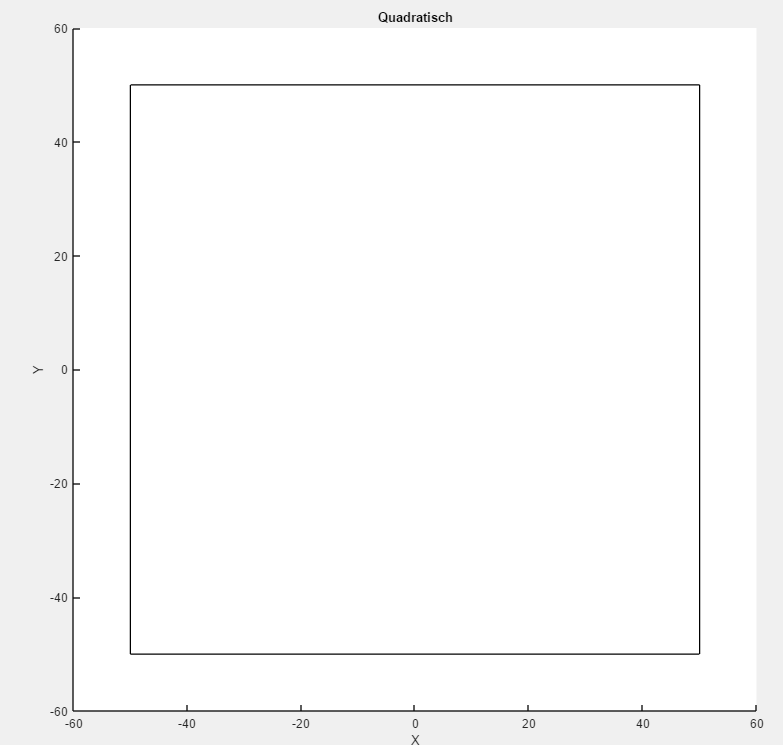
\includegraphics[width=0.32\linewidth]{Images/box.png}
	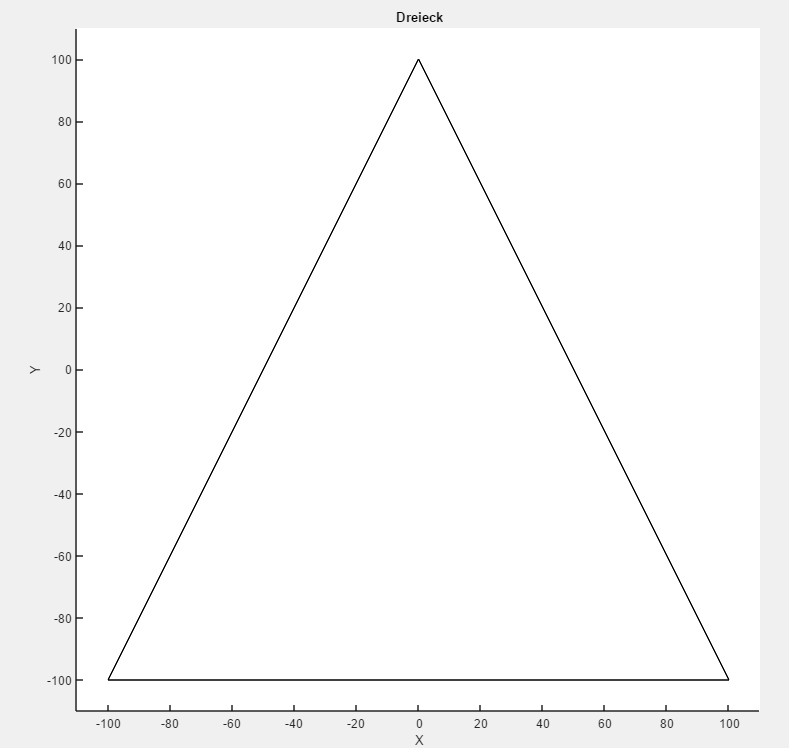
\includegraphics[width=0.32\linewidth]{Images/Dreieck.png}
	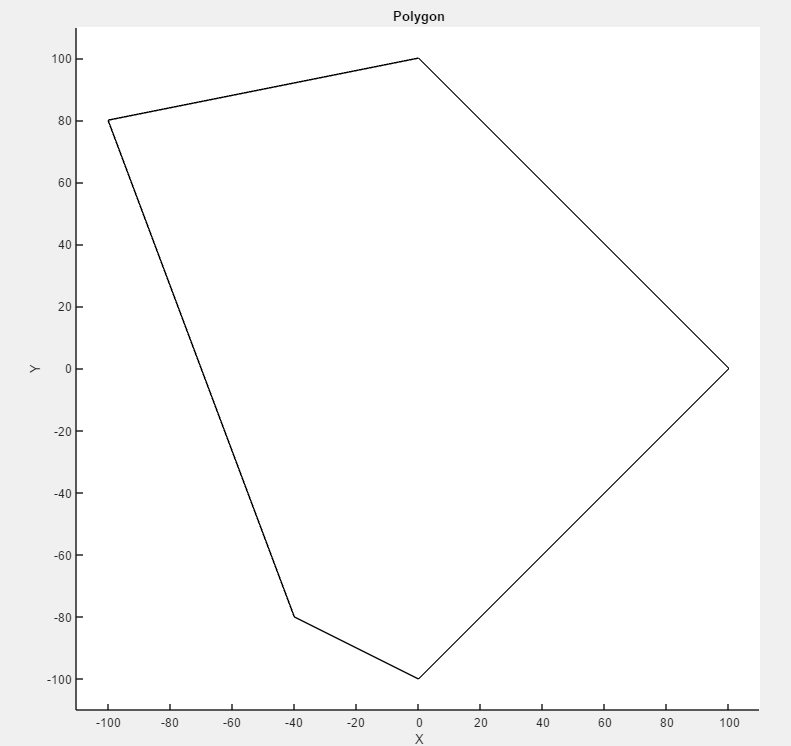
\includegraphics[width=0.32\linewidth]{Images/poly.png}
	\caption{Die drei zur Auswertung verwendeten Kartentypen}
	\label{fig:map}
\end{figure}

\begin{table}[h!]
	\centering
	\caption{Testreihen mit Anzahl Schritten}
	\label{tab:testreihen}
	\begin{tabular}{lll}
		\toprule
		Rauschen &  SE(2)-Filter &  Partikelfilter\\
		\midrule
		Normalverteilt 	& 300       & 300\\
		SE(2)-Bingham 	& 300		& 300\\
		Reale Daten 	& 60+40		& 60+40\\
		\bottomrule
	\end{tabular}
\end{table}


\subsection{Ergebnisse}

Tabelle \ref{tab:ergebnisse} stellt eine Übersicht der Evaluationsergebnisse. Die Fehlerdistanzen wurden über alle Schritte gemittelt.
Abbildung \ref{fig:gaussian} und \ref{fig:se2} zeigen den Fehlerverlauf von jeweils zwei Testreihen auf der quadratischen Karte. Hier wurde die euklidische Distanz zwischen der Position des Laufroboters und Ground Truth verwendet. Wie zu erwarten ist jeweils das Fiter-Verfahren, dessen angenommene Rauschverteilung mit der des tatsächlichen Systemmodells übereinstimmt etwas besser. Auffällig ist außerdem, dass beim SE(2)-Bingham-Rauschen der Fehler beider Verfahren deutlich größer ist.

Die Diagramme in Abbildung \ref{fig:roterror} zeigen den Rotationsfehler. Die unterschiedliche Zahl an Nulldurchgängen könnte ein Hinweis darauf sein, dass der Partikelfilter sich im Vergleich träger verhält.

Abbildung \ref{fig:real} zeigt den Positionsfehler für ein Bewegungsmuster des echten Crawlers. Die Lokalisations funktioniert deutliche schlechter, als in Simulation. Teilweise sogar gar nicht, wenn der Anfangszustand zur Initialisierung der Filter zu weit vom der tatsächlichen Position abweicht. Besonders empfindlich reagiert die Lokalisation, wenn der anfängliche Rotoationsfehler groß ist. Um einen signifikanten Unterschied zwischen den beiden Verfahren feststellen zu können, würde eine wesentlich größere Anzahl an aufgezeichneten Schritten des echten Crawler nötig werden.
Geringe Unterschiede in der Laufzeit lassen sich dennoch bemerkbar. Der Partikelfilter mit 100 Partikeln wertet die Messfunktion wesentlich häufiger aus, als der SE(2)-Filter mit dem Progressiven Update.

\begin{table}[h!]
	\centering
	\caption{Mittlere Fehler}
	\label{tab:ergebnisse}
	\begin{tabular}{lll}
		\toprule
		Rauschen &  SE(2)-Filter &  Partikelfilter\\
		\midrule
		Normalverteilt 	& 6.7       & 5.8\\
		SE(2)-Bingham 	& 7.5		&  8.8\\
		Reale Daten 	& 11.2		& 10.4\\
		\bottomrule
	\end{tabular}
\end{table}

\begin{figure}[h!]
	\centering
	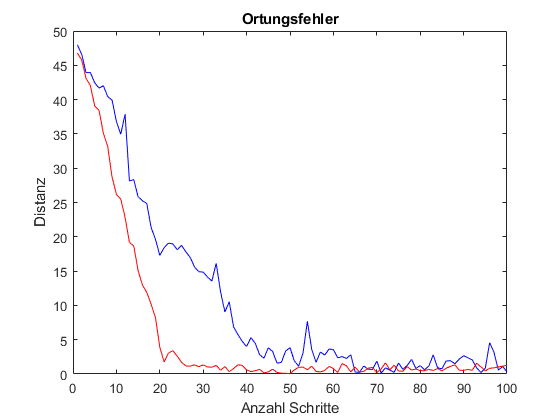
\includegraphics[width=0.7\linewidth]{Images/gaussianBox.png}
	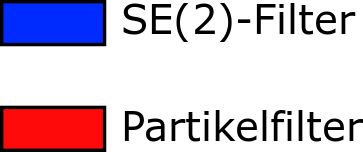
\includegraphics[width =0.1\linewidth]{Images/Legende.png}
	\caption{Normalverteiltes Rauschen}
    \label{fig:gaussian}
    
	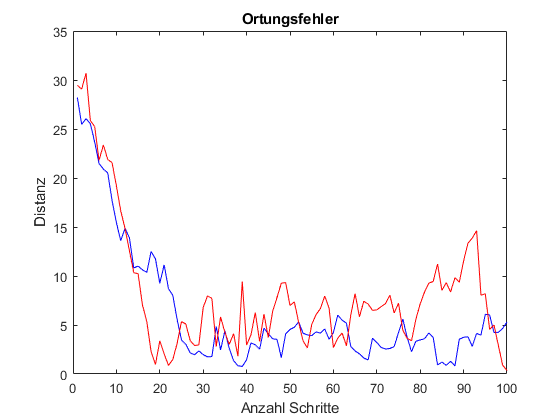
\includegraphics[width=0.7\linewidth]{Images/se2Box.png}
	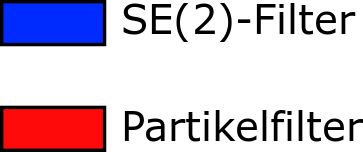
\includegraphics[width =0.1\linewidth]{Images/Legende.png}
	\caption{SE(2)-Bingham-verteiltes Rauschen}
	\label{fig:se2}
	\caption{Ergebnisse der Simulation mit Quadratischer Karte}
\end{figure}

\begin{figure}[h!]
	\centering
	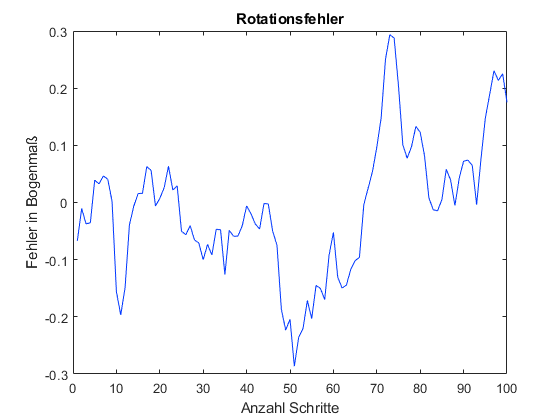
\includegraphics[width=0.40\linewidth]{Images/rotSE2.png}
	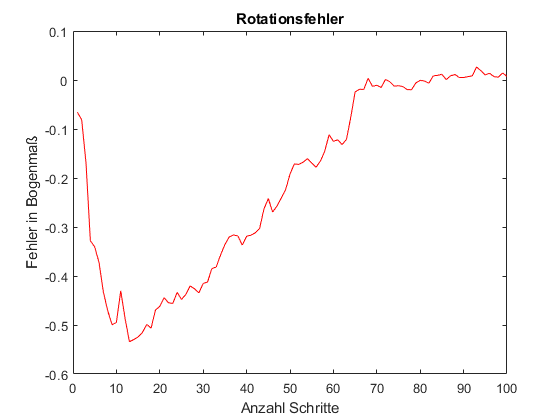
\includegraphics[width=0.40\linewidth]{Images/rotation.png}
	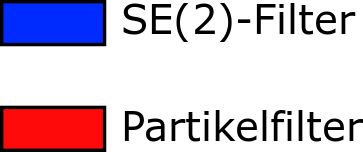
\includegraphics[width =0.18\linewidth]{Images/Legende.png}

	\caption{Rotationsfehler für quadratische Karte mit SE(2)-Bingham-Rauschen}
	\label{fig:roterror}
\end{figure}

\begin{figure}[h!]
	\centering
	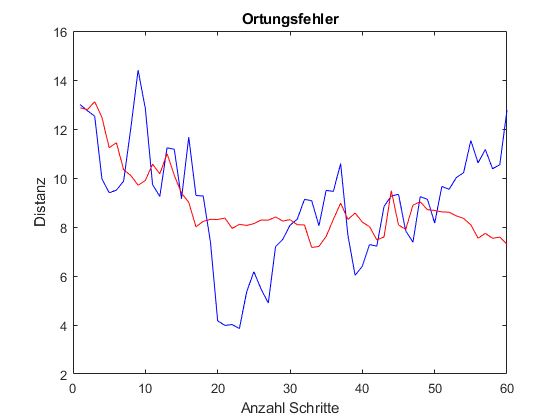
\includegraphics[width=0.60\linewidth]{Images/se2ErrorRealBoth.png}
	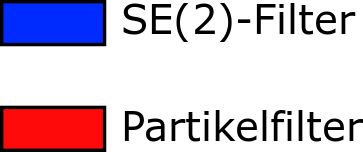
\includegraphics[width =0.18\linewidth]{Images/Legende.png}

	\caption{Fehler für die Bewegung des echten Crawlers}
	\label{fig:real}
\end{figure}

\clearpage
\section{Zusammenfassung und Ausblick}
Es wurde der SE(2)-Filter, sowie nötige Grundlagen der Schätztheorie, über Bayes-Filterung und duale Quaternionen vorgestellt. Gängige Verfahren wie der Partikel- und Kalman-Filter wurden beschrieben. Die Implementientierung des Filters, insbesondere System- und Messmodell, sowie das Progressive Update wurden erläutert. Zuletzt wurden die Ergebnisse der Evaluation des SE(2)-Filters im Vergleich zum Partikelfilter dargestellt. Es konnte kein signifikanter Unterschied zwischen den beiden Schätzmethoden festegestellt werden, dazu müssten mit größere Mengen an Bewegungsschritten des Crawlers getestet werden. Weiter mögliche Erweiterungen sind denkbar. Es können weitere Versuche mit neuen Karten vorgenommen werden. Die quadratische Karte war die einzige, mit der echte Daten gesammelt wurden. Eine komplexere Messfunktion, die die Kegelform des Ultraschallmessfelder berücksichten, würde den Crawler besser modellieren.  Nur aus den vier stark verrauschten Distanzdaten auf die Position des Laufroboters zu schließen ist ein schwieriges Problem. Es wäre interessant zu überprüfen, wie sich die Verfahren verhalten, wenn enger an die Postion gekoppelte Messgrößen beobachtet werden, zum Beispiel durch die IMU des Crawlers. In späteren Versuchen könnte man sich von der Ebene loslösen und die Lokalisation in 3D fortsetzen.
\newpage




\bibliographystyle{source}

\begin{thebibliography}{99}

\bibitem{jia2013dual}Jia, Yan-Bin (2013). Dual quaternion. Com S, 477, 577.
\bibitem{kurz2014recursive}Kurz, G., Gilitschenski, I., Julier, S.,  Hanebeck, U. D. (2014). Recursive Bingham filter for directional estimation involving 180 degree symmetry. Journal of Advances in Information Fusion, 9(2), 90-105.
\bibitem{gilitschenki2014new}Gilitschenski, I., Kurz, G., Julier, S. J.,  Hanebeck, U. D. (2014, July). A new probability distribution for simultaneous representation of uncertain position and orientation. In Information Fusion (FUSION), 2014 17th International Conference on (pp. 1-7). IEEE.
\bibitem{kurz2016Recursive}Kurz, G., Gilitschenski, I.,  Hanebeck, U. D. (2016). Recursive Bayesian filtering in circular state spaces. IEEE Aerospace and Electronic Systems Magazine, 31(3), 70-87.
\bibitem{gilitschenski2015}Gilitschenski, I., Kurz, G.,  Hanebeck, U. D. (2015, September). A stochastic filter for planar rigid-body motions. In Multisensor Fusion and Integration for Intelligent Systems (MFI), 2015 IEEE International Conference on (pp. 13-18). IEEE.
\bibitem{kurz2014}Kurz, G., Gilitschenski, I.,  Hanebeck, U. D. (2014, June). Nonlinear measurement update for estimation of angular systems based on circular distributions. In American Control Conference (ACC), 2014 (pp. 5694-5699). IEEE.
\end{thebibliography}
\end{document}
